\chapter[Sprint 1]{Sprint 1}

\section{Planejamento}

A iteração um, tinha como objetivo entregar as histórias de maior valor para o cliente. Seguindo as histórias detalhadas na iteração I (SESSAO ITERACAO 1). A imagem abaixo representa o planejamento das sprints para a release 1:

\begin{figure}[H]
    \centering
	\includegraphics[keepaspectratio=true,scale=0.35]{figuras/sprint1.eps}
    \caption{Planejamento das Sprints}
    \label{}
\end{figure}

Conclui-se pela imagem que as sprints priorizadas tinha todos o valor de negócios como must have.

\section{Desenvolvimento}

A sprint 1 foi executada com sucesso e o produto gerado segue todos os critérios de aceitação. Segue abaixo uma ilustração das histórias implementadas.

\textbf{História 7}

\begin{figure}[H]
    \centering
	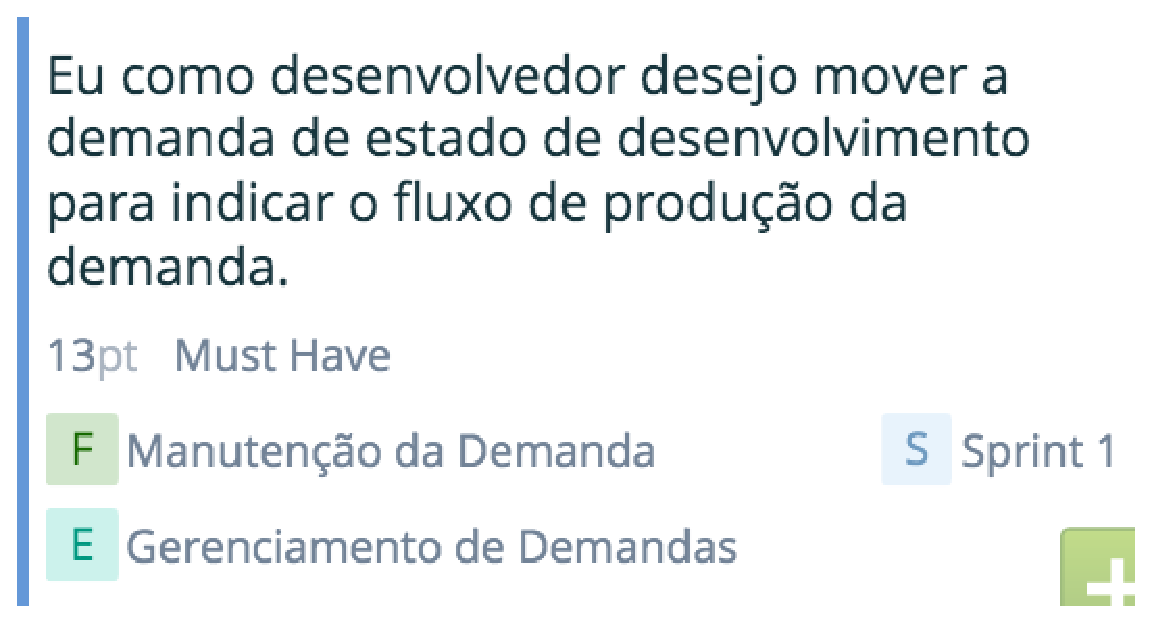
\includegraphics[keepaspectratio=true,scale=0.6]{figuras/sprint2.eps}
    \caption{História de usuário 7}
    \label{}
\end{figure}

\textbf{Critérios:}
\begin{enumerate}
	\item O desenvolvedor poderá alterar uma demanda para a fase seguinte alterando seu status .
	\item A mudança do status deve seguir o fluxo e os status.
\end{enumerate}

\begin{figure}[H]
    \centering
	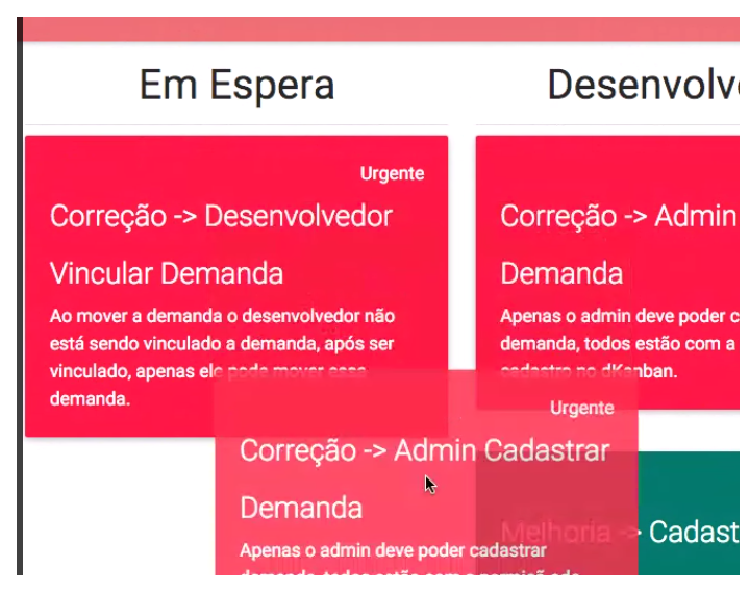
\includegraphics[keepaspectratio=true,scale=0.6]{figuras/sprint3.eps}
    \caption{Movendo demanda de desenvolvendo para em espera}
    \label{}
\end{figure}

\begin{figure}[H]
    \centering
	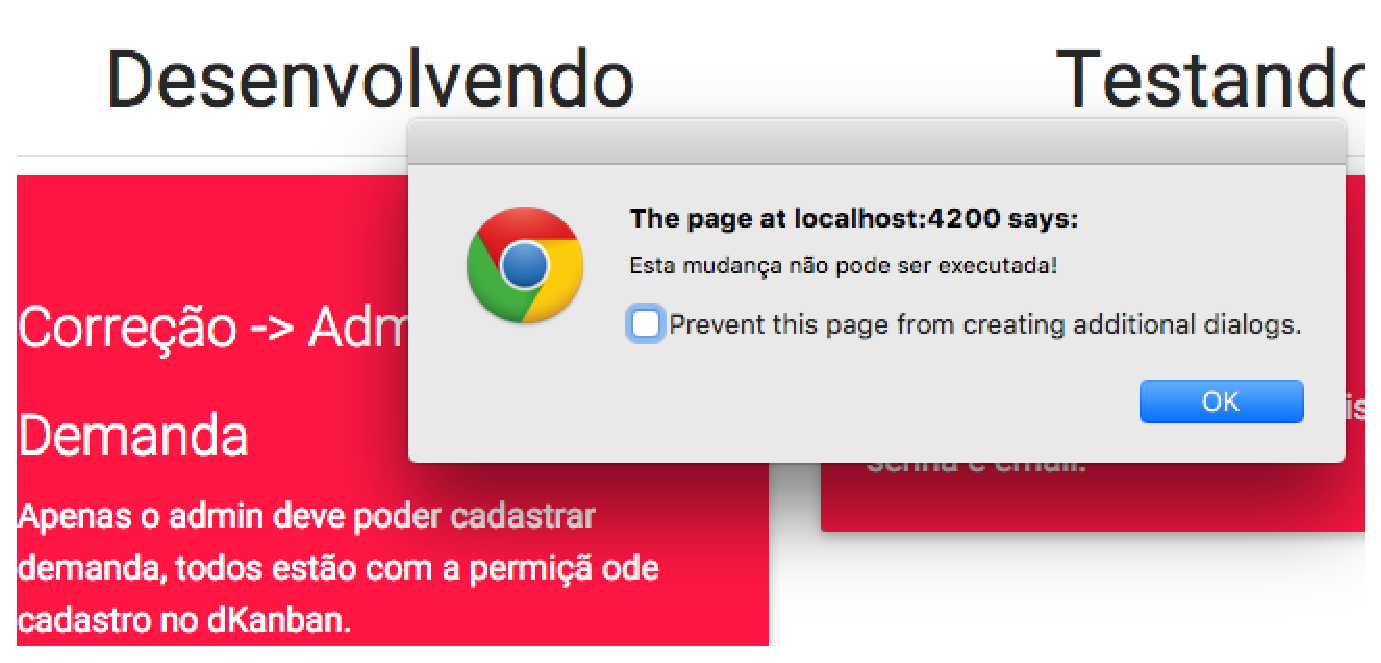
\includegraphics[keepaspectratio=true,scale=0.6]{figuras/sprint4.eps}
    \caption{Apresentando mensagem de erro}
    \label{}
\end{figure}

\begin{figure}[H]
    \centering
	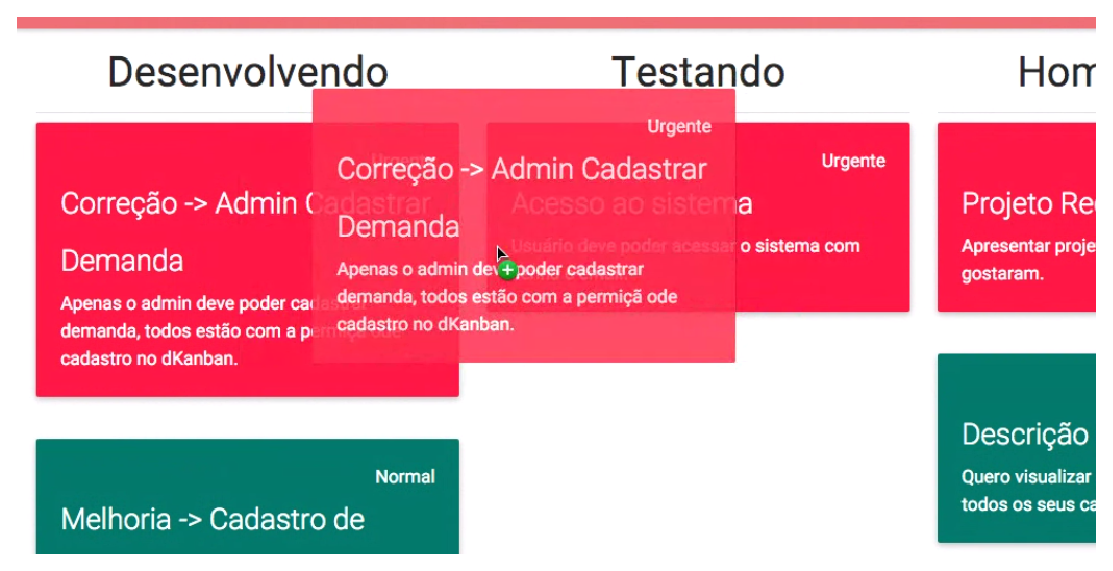
\includegraphics[keepaspectratio=true,scale=0.6]{figuras/sprint5.eps}
    \caption{Movendo demanda desenvolvendo para testando}
    \label{}
\end{figure}

\begin{figure}[H]
    \centering
	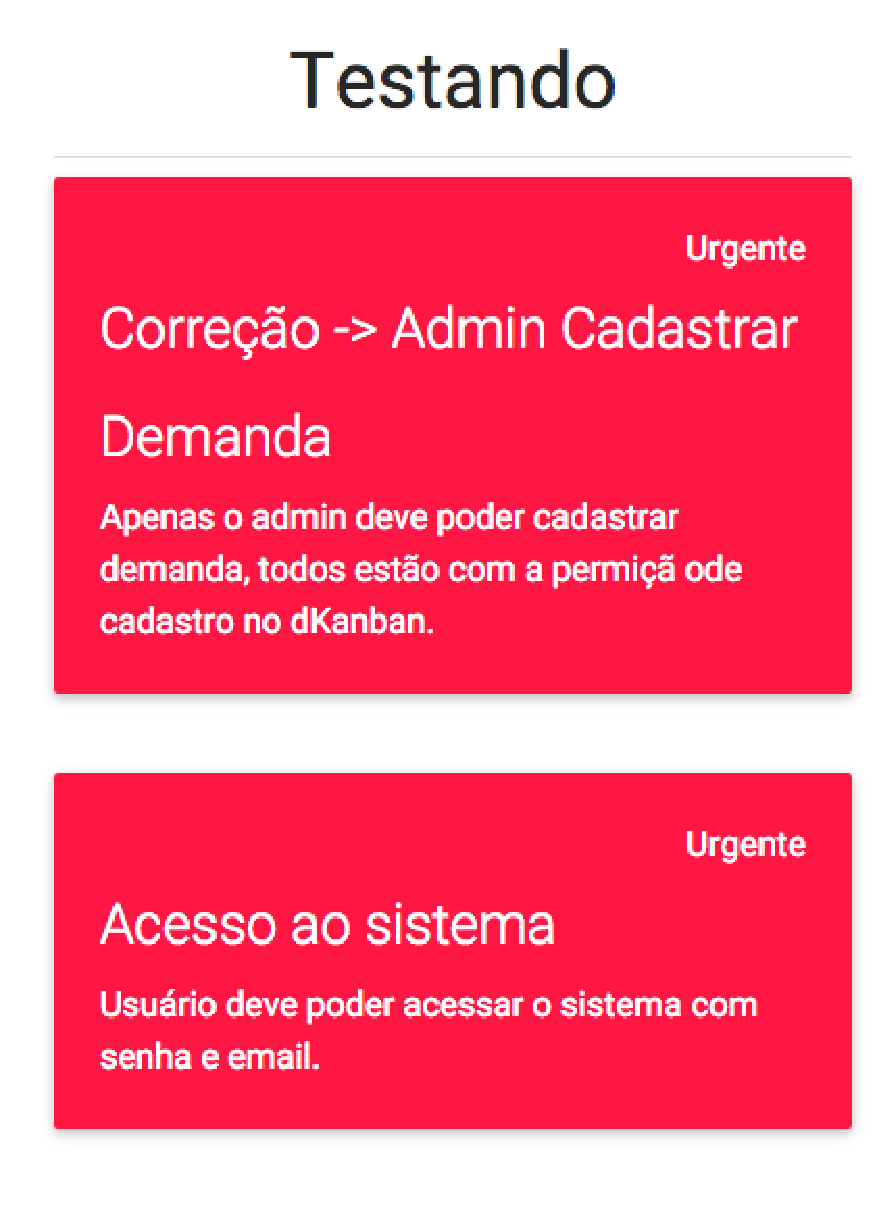
\includegraphics[keepaspectratio=true,scale=0.5]{figuras/sprint6.eps}
    \caption{Demanda movida com sucesso}
    \label{}
\end{figure}


\textbf{História 3}

\begin{figure}[H]
    \centering
	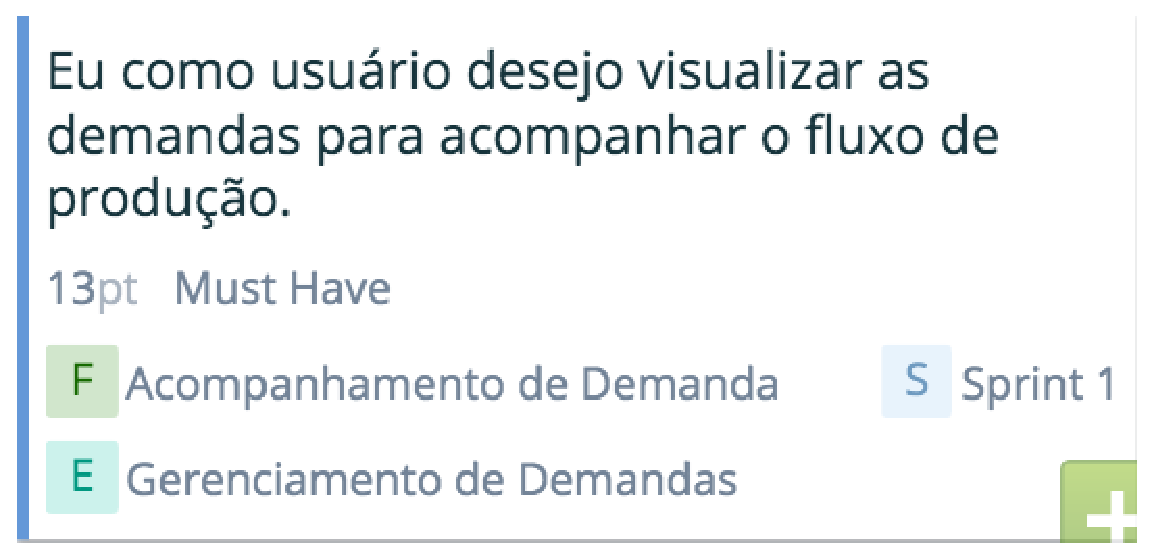
\includegraphics[keepaspectratio=true,scale=0.6]{figuras/sprint8.eps}
    \caption{História de usuário 3}
    \label{}
\end{figure}

\textbf{Critérios:}
\begin{enumerate}
	\item A demanda será ordenada por nível de prioridade.
	\item O gerente e o desenvolvedor podem visualizar todas as demandas.
\end{enumerate}

\begin{figure}[H]
    \centering
	\includegraphics[keepaspectratio=true,scale=0.3]{figuras/sprint7.eps}
    \caption{Visualização de todas as demandas priorizadas}
    \label{}
\end{figure}
